\documentclass[a4paper]{report}
\usepackage[T2A]{fontenc}
\usepackage[utf8]{inputenc}
\usepackage[russian,english]{babel}
\usepackage[pdftex]{hyperref}
\pagestyle{plain}
\usepackage{mathtext} 
\usepackage[14pt]{extsizes}
\usepackage{placeins}
\usepackage{indentfirst} 
\frenchspacing

\usepackage{enumitem}

\usepackage{titletoc}
\usepackage{setspace}
\sloppy
\usepackage{titlesec}
\titlespacing\section{1.25cm}{0cm}{12pt}
\titlespacing\subsection{1.25cm}{0cm}{12pt}

\usepackage{tocloft}
\setlength{\cftbeforetoctitleskip}{-4em}
\setlist{nosep,wide}
\setlength{\topsep}{-20pt}
\setenumerate[1]{label=\arabic*.}

\usepackage[final]{graphicx}

\usepackage[tableposition=top,singlelinecheck=false]{caption}
\usepackage{subcaption}
\DeclareCaptionLabelFormat{gostfigure}{Рис. #2}
\DeclareCaptionLabelFormat{gosttable}{Таблица #2}
\renewcommand{\labelenumii}{\arabic{enumi}.\arabic{enumii}.} 
\DeclareCaptionLabelSeparator{gost}{~---~}
\captionsetup{labelsep=gost}
\captionsetup*[table]{labelformat=gosttable, margin={1.25cm,0pt}}
\captionsetup*[figure]{labelformat=gostfigure,justification=centering}
\renewcommand{\thesubfigure}{\asbuk{subfigure}}


\usepackage[T2A]{fontenc}
\usepackage[left=3cm, right=1cm, vmargin=2cm]{geometry}

\usepackage[final]{listings}
\usepackage{xcolor}
\usepackage{caption}


\lstset{
	language=C++,                 
	basicstyle=\footnotesize, 
	numbers=left,     
	numberstyle=\tiny,       
	stepnumber=1,          
	firstnumber=1,
	numberfirstline=true
	numbersep=5pt, 
	identifierstyle=\color{gray},
	keywordstyle=\color{blue}\bfseries,
	commentstyle=\color{green},      
	stringstyle=\color{red},   
	morecomment=[l][\color{pink}]{\#},
	showspaces=false,           
	showstringspaces=false,      
	showtabs=false,             
	tabsize=4,                
	captionpos=t,              
	breaklines=true,           
	breakatwhitespace=false,
	extendedchars=true,
	frame=tb,
	title=\lstname
}


\begin{document}
	%--------------------------------------------------------------------------------
	%	ТИТУЛЬНЫЙ ЛИСТ
	%--------------------------------------------------------------------------------
	\begin{titlepage}
	
		\begin{center} 
			\par МИНИСТЕРСТВО ОБРАЗОВАНИЯ И НАУКИ РОССИЙСКОЙ ФЕДЕРАЦИИ
			\par ФЕДЕРАЛЬНОЕ ГОСУДАРСТВЕННОЕ АВТОНОМНОЕ ОБРАЗОВАТЕЛЬНОЕ УЧРЕЖДЕНИЕ 
			\par «Нижегородский государственный университет им. Н.И. Лобачевского\\[0.2cm]
			\par Национальный исследовательский университет\\[0.1cm]
			\par Институт информационных технологий, математики и механики \\[0.1cm]
			\par Кафедра математического обеспечения и суперкомпьютерных технологий\\[2.5cm]		
		\begin{center} 
		
		{\huge \bfseries Отчет \\[0.1cm]
			\Large \mdseries по лабораторной работе \\[0,1cm]
			\Large \mdseries по дисциплине «Параллельное программирование» \\[1cm]
			\Large \bfseries Сортировка Хоара с простым слиянием}\\[3cm]
		
		\begin{flushright} \large
			{Проверил} \\[0.1cm]
			{кандидат технических наук, доцент}\\[0.1cm]
			{\underline{\hspace{2,35in}} Сысоев А.В.}\\[0.1cm]
			{<<\underline{\hspace{0,25in}}>>\underline{\hspace{2,55in}}20\underline{\hspace{0,3in}}г.} \\[0.1cm]
			{Выполнил} \\[0.1cm]
			{Студент группы 381706-2} \\[0.1cm]
			{\underline{\hspace{2,1in}} Паршина С.С.} \\[0.1cm]
			{<<\underline{\hspace{0,25in}}>>\underline{\hspace{2,55in}}20\underline{\hspace{0,3in}}г.} \\[3cm]
		\end{flushright}
		
		\centering{
			Нижний Новгород\\
			\the\year { г.}
		}
	\end{titlepage}
	
	%--------------------------------------------------------------------------------
	%	АВТОМАТИЧЕСКИ СОБИРАЕМОЕ СОДЕРЖАНИЕ
	%--------------------------------------------------------------------------------
	\begin{spacing}{1.5}  
		\renewcommand{\contentsname}{\centerline{\Large{Cодержание}}}
		\dottedcontents{chapter}[1.6em]{}{1.6em}{1pc}
		\tableofcontents
		\setcounter{page}{2}
		
		\newpage
		%--------------------------------------------------------------------------------
		%	ВВЕДЕНИЕ
		%--------------------------------------------------------------------------------
		
		\centerline{\section*{Введение}}
		\addcontentsline{toc}{section}{Введение}
		
		\setlength{\parindent}{1.25cm}
		\setlength{\parskip}{8pt}
		
		\par В современном мире компьютерные системы имеют огромные вычислительные возможности. Очевидно, что в связи с возрастанием их мощностей повышаются и сложности задач, и объемы данных, которые обрабатывают данные системы. Алгоритмы сортировки, то есть упорядочивания различных объектов по какому-либо критерию, – одна из самым популярных задач в программировании. Существует огромное количество сортировок: медленных и быстрых, устойчивых и неустойчивых, внутренних и внешних. Конечно, следует учитывать, какие и в каком объеме данные сортируются, но на данный момент обсуждение сводится к тому, что быстрая сортировка Хоара является самой эффективной. Так или иначе, все больше появляется необходимость усовершенствовать этот процесс: экономно использовать память и увеличивать быстродействие. Один из основных способов уменьшения времени работы программы – использование технологий и библиотек параллельного программирования. В течение всего семестра было выполнено несколько лабораторных работ, отражающих их применение на конкретной задаче быстрой сортировки с разбиением Хоара с простым слиянием: последовательная версия, ее распараллеливание с помощью открытого стандарта OpenMP , а также с помощью библиотеки шаблонов C++, предоставленной компанией Intel для параллельного программирования – Intel Threading Building Blocks.
		
		\newpage
		%--------------------------------------------------------------------------------
		%	ПОСТАНОВКА ЗАДАЧИ 
		%--------------------------------------------------------------------------------
		
		\renewcommand*{\thesection}{\arabic{section}}
		\section{Постановка задачи}
		
		\par В данной лабораторной работе необходимо изучить алгоритм быстрой сортировки Хоара с простым слиянием отсортированных частей массива, а также рассмотреть и сравнить эффективность интеграции этого алгоритма и двух технологий параллельного программирования: OpenMP и Intel TBB. Для достижения поставленной цели необходимо выполнить следующие задачи: 
		\begin{itemize} 
			\item[--] исполнить последовательную версию алгоритма;
			\item[--] исполнить параллельную версию алгоритма с помощью стандарта OpenMP;
			\item[--] исполнить параллельную версию алгоритма с помощью библиотеки Intel TBB;
			\item[--] провести эксперименты с разными объемами массивов и количеством потоков;
			\item[--] сделать выводы об эффективности и сложности каждого способа распараллеливания, выявить зависимость скорости работы алгоритмов от объема входных данных, количества потоков и физических характеристик компьютера. 
		\end{itemize}
		
		\newpage
		
		%--------------------------------------------------------------------------------
		%	ОПИСАНИЕ АЛГОРИТМА 
		%--------------------------------------------------------------------------------
		\section{Описание алгоритма}
		
		\par Сортировка является одной из типовых проблем обработки данных и обычно понимается как задача размещения элементов неупорядоченного набора значений S = \{a1, a2 ,..., an\} в порядке монотонного возрастания или убывания (здесь и далее все пояснения для краткости будем понимать сортировку как упорядочивание элементов массива по возрастанию).
		\par Существует огромное количество алгоритмов сортировок: внутренние – оперируют массивами, целиком помещающимися в оперативной памяти с произвольным доступом к любой ячейке и внешние  – оперируют запоминающими устройствами большого объёма, но не с произвольным доступом, а последовательным (упорядочение файлов), то есть в данный момент «виден» только один элемент, а затраты на перемотку по сравнению с памятью неоправданно велики; устойчивые – не меняют относительного порядка элементов при сортировке и неустойчивые  - сортируемые элементы могут менять относительный порядок, алгоритмы, не основанные на сравнениях, сортировка вставками, обменные, посредством выбора, подсчетом и другие.
		\par Вычислительная трудоемкость процедуры упорядочивания является достаточно высокой. Так, для ряда известных простых методов (пузырьковая сортировка, сортировка включением и др.) количество необходимых операций определяется квадратичной зависимостью от числа упорядочиваемых данных T \sim $n^2$.
		\par Для более эффективных алгоритмов (сортировка слиянием, сортировка Шелла, быстрая сортировка) трудоемкость определяется величиной T \sim $nlog{}_2 n$.
		\par Данное выражение дает также нижнюю оценку необходимого количества операций для упорядочивания набора из n значений; алгоритмы с меньшей трудоемкостью могут быть получены только для частных вариантов задачи. 
		\par Главным объектом данной лабораторной работы является быстрая сортировка с разбиением Хоара и с простым слиянием отсортированных частей массива. Алгоритм быстрой сортировки данных, разработанный Чарльзом Хоаром в 1960 году, является одним из самых известных, универсальных и часто используемых алгоритмов. Алгоритм по принципу функционирования входит в класс обменных сортировок (сортировка перемешиванием, пузырьковая сортировка и так далее), выделяясь при этом высокой скоростью работы на большом количестве элементов.
		\par Отличительной особенностью именно быстрой сортировки является операция разбиения массива на две части относительно опорного (pivot) элемента. Таким образом она относится к типу сортировок <<разделяй и влавствуй>>, то есть базируется на последовательном разделении массива на блоки меньшего размера таким образом, что между значениями разных блоков обеспечивается отношение упорядоченности: все элементы из первого блока не превосходят элементы второго. Например, если последовательность требуется упорядочить по возрастанию, то в левый блок относительно опорного элемента будут перенесены значения меньше, а в правый – больше или равные него. 
		\par Таким образом, суть алгоритма сортировки выражается в двух шагах:
		
		\begin{enumerate} 
			\item разбиение массива относительно опорного элемента;
			\item рекурсивное доупорядочивание (сортировка) каждой части массива.
		\end{enumerate}
		
		\par Ключевым элементов быстрой сортировки является алгоритм переупорядочивания или разбиения. Есть несколько видов разбиения: Ломуто, Хоара. 
		\par Основные этапы разбиения Хоара:
		
		\begin{enumerate} 
			\item вводятся указатели first и last для обозначения начального и конечного элементов последовательности, а также опорный элемент pivot;
			\item вычисляется значение опорного элемента (first+last)/2, и заноситься в переменную pivot;
			\item указатель first смещается с шагом в 1 элемент к концу массива до тех пор, пока array[first]>pivot. А указатель last смещается от конца массива к его началу, пока array[last]< pivot;
			\item каждые два найденных элемента меняются местами;
			\item пункты 3 и 4 выполняются до тех пор, пока first<last.
		\end{enumerate}
		
		\par После разбиения последовательности следует проверить необходимость дальнейшего продолжения рекурсивной сортировки.
		\par Рассмотрим пример этого разбиения относительно медианного элемента: array = \{6, 7, 2, 5, 9, 1, 3, 8\}, first = 1, last = 8. Пройденная часть будет выделена жирным шрифтом.
		
		\begin{enumerate} 
			\item Индекс опорного элемента pivot = (1+8)/2 =  4,5 = 4 (отбрасывая дробную часть).  array = \{6, 7, 2, 5, 9, 1, 3, 8\}. Сравниваем слева все элементы с 5, останавливаемся на первом большем опорного элементе. array[1]>pivot, значит first = 1. Переходим в левый блок. Первый меньший 5 элемент – это 3 с индексом last = 7. Первый и седьмой элементы меняются местами. Оба указателя смещаются на единицу: один - вправо, другой – влево. array = \{\textbf{3}, 7, 2, 5, 9, 1, \textbf{6,8}\}  
			
			\item Продолжаем аналогично сравнивать элементы двух частей массива с опорным. array[2]>pivot, значит first=2. Переходим в правый блок. Находим 1, которая находится <<не в своем подмассиве>> относительно опорного элемента, значит last = 6. Меняем местами 2 и 6 элементы. Смещаем указатели на единицу и с той, и с другой стороны. array = \{\textbf{3,1,} 2, 5, 9, \textbf{7,6,8}\} 
			
			\item Продолжаем. Третий элемент меньше опорного, значит находится «на своем месте». Справа оставшийся пятый элемент больше опорного, значит его переносить также не нужно. Таким образом, first=last=4, значит условие first<last не выполняется, первый этап быстрой сортировки – разбиение Хоара, завершается. array = \{\textbf{3, 1, 2, 5, 9, 7, 6, 8}\}
		\end{enumerate}
		
		\par Разбиение завершено. Массив разделен на два блока относительно опорного элемента, слева большего опорного, справа - меньше. Можно переходить ко второму этапу сортировки – рекурсивному доупорядочиванию. 
		\par Если в какой-либо из двух блоков после разбиения осталось больше одного элемента, то необходимо произвести рекурсивное сортировку этой части, то есть аналогичным образом разбить этот блок. Проверить это условие можно с помощью следующих ограничений: если индекс начала массива меньше, чем индекс last, на \par котором остановилось разбиение справа, то доупорядочиваем левую часть. Аналогично, если индекс конца массива больше, чем индекс first, на котором остановилось разбиение слева, то доупорядочиваем правую часть. 
		Учитывая тот факт, что каждый раз элементы из левого подмассива всегда меньше, что элементы из правого, то если каждая из частей массива пройдет через процедуру разбиения, то элементы автоматически окажутся отсортированными и «обработанные» части объединяются в результирующий массив методом простого слияния. 
		\par В программном коде реализованы методы HoarePartition, который возвращает индекс самого правого элемента, на котором закончилось разбиение, и метод qHoareSort, который непосредственно реализует быструю сортировку Хоара с простым слиянием, уточняя условие наличия в подмассивах больше 1 элемента для продолжения сортировки. Полный код последовательной версии приведен в Приложении А.
		\par Что касается эффективности, то она определяется правильностью выбора опорных элементов при формировании блоков. В худшем случае, она равна O($N^2$), то есть имеет тот же порядок, что и пузырьковая сортировка. В идеальном случае, когда разделение на подмассивы происходит примерно на равные части относительно опорного элемента, тогда его трудоемкость совпадает с наиболее эффективными алгоритмами сортировки порядка $Nlog{}_2 N$. Объясним эту сложность: 2 в логарифме – разделение на 2 равные части, $Nlog{}_2 N$ – log N уровней, так как на 1 итерации N элементов, на 2 – N/2 | N/2 уровней, на 3 – N/4 N/4 | N/4 N/4 и так далее, на каждом уровне N операций. В среднем случае время выполнения алгоритма быстрой сортировки определяется выражением Tcalc = 1,4 $Nlog{}_2 N$ $\tau$.\\[0.5pt]
		
		\begin{center}
			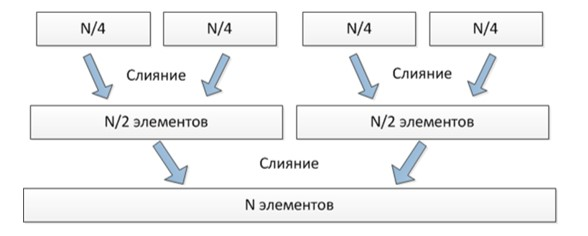
\includegraphics[width=\linewidth]{../../../../modules/reports/parshina_s_quick_sort/picture1.png}
			\captionof{figure}{Схема простого слияния} \\[0.5pt]
		\end{center}
		
		\par Если размер сортируемого массива велик настолько, что массив не может быть полностью помещен в кэш, то по мере выполнения последовательного алгоритма быстрой сортировки будет происходить чтение данных из оперативной памяти в кэш. Количество чтений определяется порядком выполнения итераций алгоритма и разницей в объеме данных для сортировки и объеме кэш. При построении оценки сверху считается, что необходимо выполнить чтение всего сортируемого массива из оперативной памяти в кэш на каждой итерации алгоритма быстрой сортировки. Время на обращение к оперативной памяти: 
		Tmem = 1,4 
		$N log{}_2 N$ (8N/$\beta$). 
		\par То есть общее время выполнения последовательного алгоритма быстрой сортировки: T = 1,4$N log{}_2 N$ \tau + 1,4 $N log{}_2 N$ (8N/$\beta$). 
		\par Рассмотрим <<плюсы>> и <<минусы>> алгоритма быстрой сортировки Хоара. Достоинства:
		\begin{itemize} 
			\item[--] объективно один из самых быстродействующих внутренних алгоритмов сортировки;
			\item[--] емкий, запоминающийся алгоритм, который нетрудно восстановить по памяти в любой момент времени;
			\item[--] улучшенная версия требует всего O(logN) дополнительной памяти;
			\item[--] хорошо сочетается с механизмом виртуальной памяти и кэширования;
			\item[--] допускает эффективную модификацию для сортировки по нескольким ключам;
			\item[--] допускает сортировку выделенных подмассивов в параллельно выполняющихся подпроцессах;
			\item[--] работает на связных списках и других структурах с последовательным доступом, допускающих эффективный проход как от начала массиву к концу, так и в обратную сторону. 
		\end{itemize}
		
		\par Недостатки:
		\begin{itemize}
			\item[--] неустойчивый алгоритм;
			\item[--] в худшем случае сильная «просадка» по скорости выполнения до O($N^2$) при неудачных входных данных;
			\item[--] прямая реализация в виде функции с двумя рекурсивными вызовами может привести к переполнению стека, потому что в худшем случае ей может потребоваться сделать O(N) вложенных рекурсивных вызовов.
		\end{itemize}
		\par Анализ показывает, что есть массив имеет до 12 элементов, то лучше использовать сортировку вставками. 
		\par Алгоритм поддается улучшению, которое направлено на устранение недостатков быстрой сортировки, то есть переквалификация алгоритма в устойчивый, устранение деградации в скорости работы и защита от переполнения стека вызовов из-за большой глубины рекурсии. В число мер входит расширение ключа исходным индексом элемента в массиве, но при этом потребуется дополнительно O(N) памяти и один полный проход по массиву для сохранения исходных индексов, выбор среднего элемента, медианы из трех элементов (первого, среднего и последнего) или случайно, создание одной ветви рекурсии вместо двух только для меньшего подмассива, а больший обрабатывается в цикле в пределах этого же вызова процедуры.
		
		\newpage
		%--------------------------------------------------------------------------------
		%	ОПИСАНИЕ СХЕМЫ РАСПАРАЛЛЕЛИВАНИЯ
		%--------------------------------------------------------------------------------
		\section{Описание схемы распараллеливания}
		
		\par Параллельное обобщение алгоритма быстрой сортировки может быть получено, если топология коммуникационной сети будет эффективно представлена в виде N-мерного гиперкуба, т.е. когда p=$2^N$, где p – число процессов. Исходный набор данных логически разделен на 2p блоков одинакового размера n/2p. Тогда первая итерация алгоритма состоит в следующем:
		\begin{itemize}
			\item[--] разделить исходный массив размером n на p частей и разослать каждому процессу его часть, выполняя сортировку каждой части с помощью быстрой сортировки;
			\item[--] выбрать определенным образом опорный элемент – в разбиении Хоара это средний элемент ведущего процесса, рассылаем этот элемент по остальным процессам. Если выбирать таким образом ведущий элемент, то в отдельных случаях это может оказаться более близким к реальному среднему значению всего сортируемого набора, чем произвольно выбранное значение;
			\item[--] разделить данные каждого процесса на элементы, меньшие значению опорного и больше или равные опорному;
			\item[--] образовать  пары процессов, для которых битовое представление номера отличается только в старшем бите (позиции N) и произвести взаимный обмен между этими процессами: процесс, который в данной позиции имеет бит, равный нулю, получает от другого элементы, меньшие опорного и отдает часть своих элементов, которые больше него. После передачи обе части сливаются. Процесс простого слияния имеет линейную от размера блока данных процесса сложность.  
		\end{itemize}
		
		\par Таким образом, на каждой итерации набор данных процесса остается упорядоченным. После первой итерации общий гиперкуб разбивается на два под-куба, процессы одной части которого содержат элементы, меньше опорного (в битовом представлении номеров в позиции N оказывается 0), а процессы другой части будут иметь элементы, большие или равные опорному. Очевидно, что общий гиперкуб из p процессоров размерности N разделился на два гиперкуба по p/2 процессоров размерности N-1. 
		\par Описанная схема далее применяется рекурсивно для полученный под-кубов. Однако, теперь можно изменить реализацию алгоритма и отказаться от рекурсивного метода, применяя итеративную схему: пары на i-той итерации образуют процессы, чьи номера в битовом представлении отличаются только в i-той позиции.  
		\par На второй итерации разделение гиперкубов продолжится (каждый еще на два), при этом новые опорные элементы выбираются как средние элементы каждого из ведущих процессов новых гиперкубов (они обладают наименьшим номером). Первый под-гиперкуб из четырех содержит элементы, меньшие опорного в первой итерации и меньше опорного во второй итерации для данного куба, при этом он меньше первого опорного элемента. Аналогично происходит и для других гиперкубов. Очевидно, что после N итераций для получения упорядоченного массива останется собрать отсортированные блоки данных с каждого процесса в порядке возрастания их номеров. 
		\par Продемонстрируем на примере работу параллельного алгоритма быстрой сортировки Хоара с простым слиянием:
		\par Пусть p=4 – количество процессов.\\[0.5pt]
		
		\begin{center}
			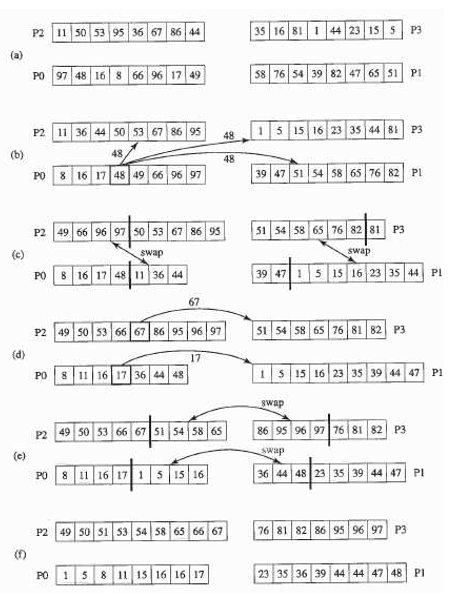
\includegraphics[width=\linewidth]{../../../../modules/reports/parshina_s_quick_sort/picture2.png}
			%\includegraphics[width=0.6\textwidth]{spiral}
			\captionof{figure}{Демонстрация работы параллельного алгоритма быстрой сортировки Хоара} \\[0.5pt]
		\end{center}
		
		\par Оценим эффективность параллельного алгоритма быстрой сортировки. Пусть дано p процессоров p = $2^N$, n – размер сортируемого массива. N – известное число итераций параллельного алгоритма.
		\par Предполагается, что на каждой итерации выбирается опорный элемент наиболее удачным способом и размер пересылаемых частей всегда одинаков и равен n/2p. При этом размер блока данных каждого процесса на каждой итерации одинаков и равен n/p. Перед началом работы алгоритма каждый процессор выполняет сортировку своего блока данных. При использовании быстрой сортировки оценка числа операций n/p $log{}_2$ (n/p) * $\tau$ , 
		где $\tau$ – время выполнения элементарной операции перестановки элементов в массиве.
		\par На каждой из N = $log{}_2$p итераций каждый процессор выполняет разделение своего блока данных по опорному элементу. Так как блок данных упорядочен, то это разделение можно провести путём поиска опорного элемента в этом блоке двоичным поиском, оценка числа операций для поиска: $log{}_2$ (n/p).
		\par Также на каждой итерации происходит слияние двух блоков данных: оставшегося на процессоре и принятого от другого процессора. Размеры обоих этих блоков равны по n/2p и, таким образом, оценка числа операций для процедуры слияния двух частей n/p * $\tau$.
		\par Так как обе эти операции выполняются на каждой из N = $log{}_2$(p) итераций, то в общую оценку они входят с множителем N. Таким образом, общее время вычислений параллельного алгоритма быстрой сортировки составляет:
		Tp(calc) = $\tau$ [n/p $log{}_2$ (n/p) + $log{}_2$ p(n/p+$log{}_2$(n/p))]
		\par Теперь оценим сложность выполняемых коммуникационных операций. Общее количество межпроцессных обменов для рассылки ведущего элемента на N-мерном гиперкубе может быть ограничено оценкой: 
		\sum_{i=1}^N N*(N+1)/2 = $log{}_2 $ p ($log{}_2 $ p + 1)/2 
		\sim $($log{}_2$ p)^2$.
		
		\par Кроме того, на каждой из N = $log{}_2$ p итераций происходит пересылка n/2p элементов между каждой парой процессов, тогда коммуникационная сложность параллельного алгоритма быстрой сортировки: 
		Tp(comm) = $($log{}_2$p)^2$ ($\alpha$ + $\omega$ / $\beta$) 
		+ $log{}_2$ p ($\alpha$ + $\omega$ * n/p) / $\beta$), где $\alpha$ – латентность, $\beta$ – пропускная способность сети, $\omega$ – размер элементарного набора в байтах. 
		\par Результирующая временная сложность алгоритма быстрой сортировки: Tp = Tp(calc) + Tp(comm).
		
		\newpage
		%--------------------------------------------------------------------------------
		%	ОПИСАНИЕ ПРОГРАММНОЙ РЕАЛИЗАЦИИ
		%--------------------------------------------------------------------------------
		\begin{spacing} {0.5}
			\section{Описание программной реализации}
		\end{spacing}
		\subsection{Описание OpemMP версии}
		
		\par Одним из наиболее популярных средств программирования для компьютеров с общей памятью, базирующихся на традиционных языках программирования и использовании специальных комментариев, в настоящее время является технология OpenMP. За основу берётся последовательная программа, а для создания её параллельной версии пользователю предоставляется набор директив, функций и переменных окружения. 
		\par Предполагается, что создаваемая параллельная программа будет переносимой между различными компьютерами с разделяемой памятью, поддерживающими OpenMP API.
		\par Технология OpenMP нацелена на то, чтобы пользователь имел один вариант программы для параллельного и последовательного выполнения. Однако возможно создавать программы, которые работают корректно только в параллельном режиме или дают в последовательном режиме другой результат. Более того, из-за накопления ошибок округления результат вычислений с использованием различного количества нитей может в некоторых случаях различаться.
		\par Разработкой стандарта занимается некоммерческая организация OpenMP ARB (Architecture Review Board), в которую вошли представители крупнейших компаний – разработчиков SMP-архитектур и программного обеспечения. OpenMP поддерживает работу с языками Фортран и Си/Cи++. Первая спецификация для языка Фортран появилась в октябре 1997 года, а спецификация для языка Си/Cи++ – в октябре 1998 года. На данный момент последняя официальная спецификация стандарта – OpenMP 3.0 (принята в мае 2008 года).
		
		\par Интерфейс OpenMP задуман как стандарт для программирования на масштабируемых SMP-системах (SSMP, ccNUMA и других) в модели общей памяти (shared memory model). В стандарт OpenMP входят спецификации набора директив компилятора, вспомогательных функций и переменных среды. 
		\par OpenMP реализует параллельные вычисления с помощью многопоточности, в которой «главный» (master) поток создает набор «подчиненных» (slave) потоков, и задача распределяется между ними. Предполагается, что потоки выполняются параллельно на машине с несколькими процессорами, причём количество процессоров не обязательно должно быть больше или равно количеству потоков.
		Для использования механизмов OpenMP нужно скомпилировать программу компилятором, поддерживающим OpenMP, с указанием соответствующего ключа.
		\par При использовании OpenMP предполагается SPMD-модель (Single Program Multiple Data) параллельного программирования, в рамках которой для всех параллельных нитей используется один и тот же код.
		\par Программа начинается с последовательной области – сначала работает один процесс (нить), при входе в параллельную область порождается ещё некоторое число процессов, между которыми в дальнейшем распределяются части кода. По завершении параллельной области все нити, кроме одной (нити мастера), завершаются, и начинается последовательная область. В программе может быть любое количество параллельных и последовательных областей.
		\par Кроме того, параллельные области могут быть также вложенными друг в друга. В отличие от полноценных процессов, порождение нитей является относительно быстрой операцией, поэтому частые порождения и завершения нитей не так сильно влияют на время выполнения программы.
		
		\par Для написания эффективной параллельной программы необходимо, чтобы все нити, участвующие в обработке программы, были равномерно загружены полезной работой. Это достигается тщательной балансировкой загрузки, для чего предназначены различные механизмы OpenMP.
		\par Существенным моментом является также необходимость синхронизации доступа к общим данным. Само наличие данных, общих для нескольких нитей, приводит к конфликтам при одновременном несогласованном доступе. Поэтому значительная часть функциональности OpenMP предназначена для осуществления различного рода синхронизаций работающих нитей.
		\par OpenMP не выполняет синхронизацию доступа различных нитей к одним и тем же файлам. Если это необходимо для корректности программы, пользователь должен явно использовать директивы синхронизации или соответствующие библиотечные функции. При доступе каждой нити к своему файлу никакая синхронизация не требуется.
		\par Рассмотрим применение данной технологии к задаче быстрой сортировки. Так как OpenMP позволяет собственноручно распределять задачи и данные на потоки, то было принято решение сосредоточить все возможности технологии не на процессе сортировки, а именно на процессе простого слияния уже отсортированных последовательно частей массива, так как технология нам предоставляет возможность самостоятельно распределить относительно равные части массива на потоки, отсортировать последовательно на каждом потоке, а затем слить параллельно уже отсортированные элементы в один упорядоченный массив. 
		\par Полный код OpenMP версии представлен в приложении А. 
		\par Для корректной работы алгоритма нужно подключить директиву \#include <omp.h>
		
		\par Пройдем по основным методам и объясним логику написания программного кода: 
		
		\begin{enumerate} 
			\item 
			\par void Simple\_Fusion(double * arr, int n, int m) – метод, в котором осуществляется слияние двух уже отсортированных частей массив в один упорядоченный массив.
			\par Слияние осуществляется таким образом: пока текущий индекс первого массива меньше его размера и текущий индекс второго меньше его размера while ((a\_index < n) && (b\_index < m)), то «достаем» текущий элемент из первого массива, сравниваем с текущим элементом из второго и если первый меньше второго if (a[a\_index] < b[b\_index]), то в результирующий массив добавляем меньший элемент из соответствующего массива, то есть из первого. Также учтен случай, когда размер одного массива не равен размеру другого. Тогда мы отделяем указатель на начало оставшегося массива и его размер double \* tmp и int tmp\_max, уточняя какой именно массив больше по размеру и, соответственно, чей «конец» нужно записать в конец результирующего массива (если текущий индекс первого массива равен его размеру, то осталось во втором, и наоборот). Затем используя дополнительный цикл прохода по «остатку» for (; tmp\_index < tmp\_max; ++tmp\_index) \{ result[tmp\_index + delta] = tmp[tmp\_index] \}, записываем всегда в конец результата оставшиеся элементы из нужного массива.
			
			\item
			\par std::vector<int> Get\_Ends(int thread\_num, int n, int threads\_value) – метод, который по количеству потоков threads\_value, номеру передаваемого потока thread\_num и количеству элементов n разбивает массив на подмассивы для каждого потока и возвращает концы ends этих отрезков.
			\par Длина отрезка на каждый поток определяется, как округленный результат деления количества элементов на число потоков int sub\_length = round(1.0 * n / threads\_value). Для последнего потока и всех, кроме него разработаны различные формулы для получения начала и конца отрезка для данного потока.
			Например, если 9 элементов нужно разделить на 4 потока:
			\par 0 1 2 3 4 5 6 7 8 – индексы элементов
			\par Длина отрезка – 9/4 = 2,25 = 2 (округляя по математическим правилам)
			\par 0 поток – [0 1]
			\par 1 поток – [2 3]
			\par 2 поток – [4 5]
			\par 3 поток – [6 7 8]
			
			\item 
			\par void Parallel\_Division Sort(double * arr, int n, int threads\_value) – основной метод параллельной быстрой сортировки Хоара с простым слиянием.
			\par Для начала необходимо задать количество потоков с помощью стандартного метода omp\_set\_num\_threads(threads\_value). Инициализируем вектор векторов splitted\_ends, в котором количество векторов (строк) внутри равно числу потоков, а в каждой строке, то есть для каждого потока, располагается вектор – отрезок «начальный индекс; конечный индекс», который будет обрабатываться конкретно этим потоком. Соответственно при проходе в цикле каждому потоку «назначается в работу» с помощью метода Get\_Ends часть массива. for (int i = 0; i < threads\_value; ++i) {splitted\_ends[i] = Get\_Ends(i, n, threads\_value);}. 
			\par Входим в параллельную область с помощью директивы \#pragma omp parallel. Определяем номер текущего  потока с помощью стандартного метода int thread\_num = omp\_get\_thread\_num() и каждый отрезок отправляем в последовательную быструю сортировку qHoareSort(arr, splitted\_ends[thread\_num][0], splitted\_ends[thread\_num][1]). После этого для синхронизации и избежания гонки потоков, каждый поток должен дождаться другого потока и к выполнению следующего кода они должны приступить все вместе. Это достигается с помощью директивы \#pragma omp barrier. 
			\par Приступим к параллельному слиянию отсортированных отрезков. Определяем количество подотрезков в splitted\_ends и складываем в переменную int length = splitted\_ends.size(). Это действие понадобится в дальнейшем, так как реальную память при слиянии отсортированных отрезком мы не изменяем, а уменьшаем length в 2 раза, когда отрезки сливаются. Для этого и нужно затем проверять условие и выполнять последующий код, пока выполняется условие while (length>1). При входе в цикл с предусловием назначаем число потоков omp\_set\_num\_threads(length $/$ 2). Проиллюстрируем это действие на примере:
			\par [0 2] [3 5] [6 7] [9 11] [12 14] [15 17]
			\par Изначально 3 потока:
			\par 1 поток сливает [0 2] [3 5] -> [0 5]
			\par 2 поток сливает [6 11]
			\par 3 поток сливает [12 17]
			\par Следующий «проход»: 3/2 = 1 (округляя) поток
			\par [0 5] [6 17]
			\par Следующий «проход»: 2/2 = 1 (округляя) поток
			\par [0 17]
			\par Входим в параллельную область для параллельного слияния отсортированных частей массива. Определяем номер текущего потока int thread\_num = omp\_get\_thread\_num(). Затем создаем еще один вектор векторов std::vector<std::vector<int>> individual\_thread\_arr(2). Его размер 2 – количество подотрезков, которые сливаются. Сама эта переменная – индивидуальная переменная для каждого потока для хранения концов, с которым данный поток работает. Другими словами, это знание для каждого потока о том, какие 2 отрезка он сливает: [a; b] [b+1; c]. 
			\par Задаем переменную начала «слития» int first\_sub\_section = thread\_num * 2 + (length \% 2), int second\_sub\_section = first\_sub\_section + 1 – конец <<слития>>. Задаем individual\_thread\_arr[0] = splitted\_ends[first\_sub\_section], individual\_thread\_arr[1] = splitted\_ends[second\_sub\_section]. Например, [0 1] – для 0 потока длины 2, [2 3] – для 1 потока длины 2. В переменной int delta = individual\_thread\_arr[0][0] в соответствии с нашим примером будет лежать a, n = individual\_thread\_arr[0][1] - individual\_thread\_arr[0][0] + 1 $//$ b-a+1, m = individual\_thread\_arr[1][1] - individual\_thread\_arr[1][0] + 1 $//$c-b-1+1 = c-b. 
			\par Сливаем отрезки, используя вышеприведенный метод Simple\_Fusion(arr + delta, n, m). Например, 
			\par [0 99] [100 199] [200 299] m=n=100
			\par [0 99] [100 299] [200 299] n=100 m=200
			\par [0 299] [100 299] [200 299] – первый отрезок – результат. Этот прием имелся в виду, когда говорилось, что реальную память при слиянии отсортированных отрезком мы не изменяем, а уменьшаем length в 2 раза при cлиянии. 
			\par Снова с помощью \#pragma omp barrier «заставляем» потоки дождаться друг друга. 
			\par Теперь нужно осуществить операцию, показанную на примере выше с помощью операции individual\_thread\_arr[0][1] = individual\_thread\_arr[1][1]. 
			\par [0 99] [100 199] [200 299] – splitted\_ends
			\par [100 199] [200 299] -  individual\_thread\_arr
			\par Simple\_fusion
			\par Нужно изменить splitted\_ends, individual\_thread\_arr становится [100 299] [200 299]. splitted\_ends =  [0 99] [100 299] [200 299]
			\par Затем в splitted\_ends на индекс insrt\_pos помещаем individual\_thread\_arr[0]. Объясним происхождение insert\_pos на примере:
			\par 1.	[0 3] [4 7] [8 11] [12 15] [16 19] [20 22]
			\par Количество неслитых отрезков l и оно четное = 6, потоков l/2 = 3
			0 поток сливает 0 и 1 отрезок, 1 поток вставляет 2 и 3 отрезок, 2 поток сливает 4 и 5 отрезок, 0 поток ставит на 0 место, 1 – на 1, 2 – на 2. 
			\par first = 2n, second = first+1
			\par inserted\_pos = n, l$/$=2
			\par 2.	Если количество неслитых отрезков l нечетное, количество потоков (int) (l$/$2). 
			\par 0 поток сливает 0 и 1 отрезок, 1 поток сливает 2 и 3 отрезок, 2 поток сливает 4 и 5 отрезок, 3 поток сливает 6 и 7. 0 поток вставляет на 1 место, 1 – на 2, 2 – на 3 (зависимость n-1). 
			second =  2n+2, first = last-1 = 2n+1
			\par Итого, first = (n-1)*2 + (length\%2), second = first+1+(length\%2), то есть inserted\_pos = (n+1) - ! (length\%2). 
			\par Снова с помощью \#pragma omp barrier «заставляем» потоки дождаться друг друга. 
			\par И окончательно уменьшаем длину массива в 2 раза и проверяем условие length>1. Например, чтобы 9 отрезков 4 потока сливают по 2. Изначально 9 отрезков, затем 5, 3, 2, 1 – эти значения удовлетворяют преобразованию length = (length + 1) $/$ 2.
			\par Полный код OpenMP версии представлен в приложении А.
			
		\end{enumerate}
		
		\subsection{Описание TBB версии}
		
		\par Intel Threading Bilding Blocks - библиотека для разработки кроссплатформенных, хорошо масштабируемых, многофункциональных программ для систем с общей памятью, разработанная компанией Intel. OpenMP позволяет программировать непосредственно в потоках. TBB написан в классах и шаблонах С++, то есть позволяет программировать в объектах. Таким образом, оказывается скрыта работа с потоками, упрощая создание параллельных программ и позволяя абстрагироваться от парадигм многопоточного программирования, позволяя сосредоточиться на решении прикладной программы. 
		\par OpenMP был разработан для FORTRAN, подход к структурам данных соответствующий. Поэтому для современного С++ гораздо лучше использовать TBB. В TBB глобальными конфликтами управлять невозможно, пулы потоков не могут быть использованы в качестве сбалансированных исполнителей задач. Оба управляют параллелизмом на уровне отдельных алгоритмов, что приводит к тому, что данные повторно передаются для каждого потока - возникает конфликт потоков, который приводит к перегрузке кэша. 
		\par TBB представляет гораздо больше шансов использовать параллелизм в областях, отличных от циклов, то есть нецикличный код лучше реализовывать с помощью Intel TBB.
		
		\begin{center}
			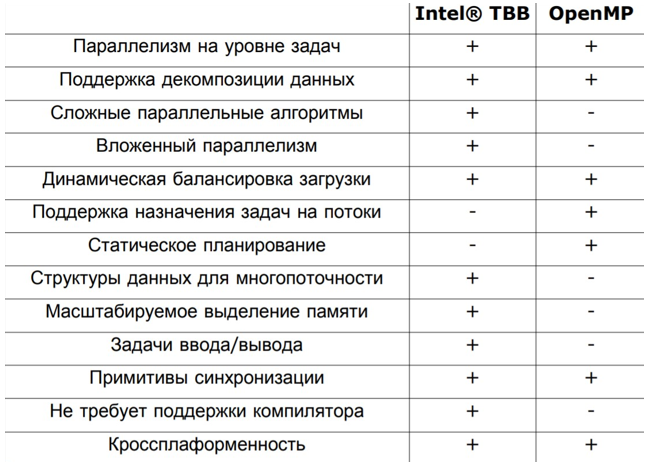
\includegraphics[width=\linewidth]{../../../../modules/reports/parshina_s_quick_sort/picture3.png}
			%\includegraphics[width=0.6\textwidth]{spiral}
			\captionof{figure}{Сравнение технологий OpenMP и Intel TBB} \\[0.5pt]
		\end{center}
		
		\par Алгоритм быстрой сортировки относится к fork-join алгоритмам (шаблонам), когда запускается исполнение нескольких задач одновременно и затем дожидается завершения каждой из них. Он удобен в применении для функциональной и рекурсивной декомпозиции и является базовым блоком для построения других шаблонов. К этому виду шаблонов также относятся сортировка слиянием, быстрая сортировка, другие алгоритмы «разделяй и влавствуй». 
		\par Часть «магии» TBB для быстрой сортировки заключается в осознании того, что, когда разделяется параллельный диапазон, можно свободно корректировать данные в этом диапазоне, прежде чем рассматривать их разделение и передавать его. Это безопасно делать, потому что когда диапазон разделяется, нет никакого параллельного использования на этом конкретном диапазоне.
		\par В планировании задач поток «отбирает» себе задачу из пула готовых к выполнению задач. Если пул пустой, приходится «воровать» из другого потока. То есть планировщик задач, встроенный в TBB, заставляет каждый поток выполнять очень простую работу: собирать работу из локального пула задач и разбивать ее, если она считается разделяемой; в противном случае он сортирует ее. Если локальная очередь задач пуста, поток пытается украсть ее из другой очереди. 
		\par Кража задачи смещается в сторону кражи из «холодного конца» пула задач, чтобы оставить позади работу, которая, скорее всего, будет иметь данные в кэше другого потока. Пул готовых к выполнению задач используется, как «последний вошел-первый вышел», но кража происходит по схеме «первый вошел-первый вышел». Это помогает избежать падения кэша и, как правило, отдает приоритет перемещению больших кусков работы за один раз. 
		\par Рассмотрим принцип, описанный выше, на известном нам алгоритме быстрой сортировки Хоара с простым слиянием на 4 потоках:
		
		\begin{center}
			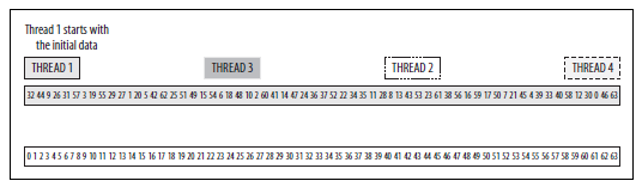
\includegraphics[width=\linewidth]{../../../../modules/reports/parshina_s_quick_sort/picture4.png}
			\captionof{figure}{Вся работа начинается с первого потока} \\[0.5pt]
		\end{center}    
		
		\begin{center}
			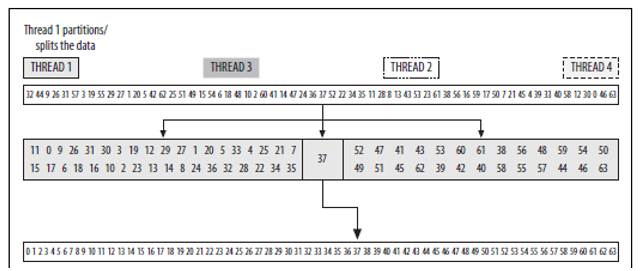
\includegraphics[width=\linewidth]{../../../../modules/reports/parshina_s_quick_sort/picture5.png}
			\captionof{figure}{Первый поток разделяет нагрузку} \\[0.5pt]
		\end{center}    
		
		\begin{center}
			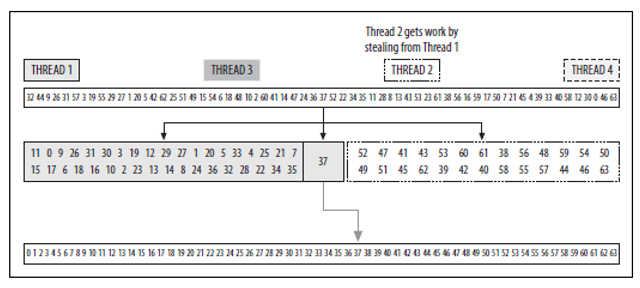
\includegraphics[width=\linewidth]{../../../../modules/reports/parshina_s_quick_sort/picture6.png}
			\captionof{figure}{Второй поток <<ворует>> работу для себя} \\[0.5pt]
		\end{center}
		
		\begin{center}
			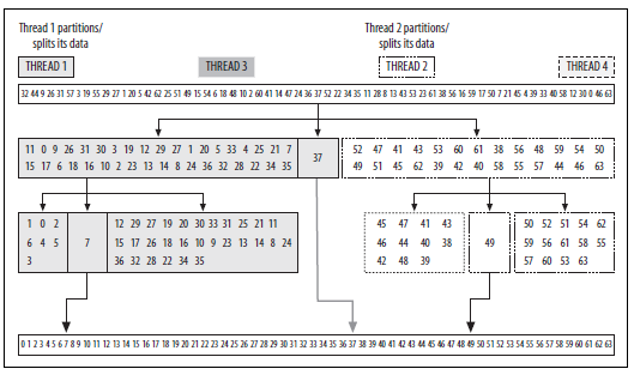
\includegraphics[width=\linewidth]{../../../../modules/reports/parshina_s_quick_sort/picture7.png}
			\captionof{figure}{Первый и второй потоки разделили нагрузку} \\[0.5pt]
		\end{center}    
		
		\begin{center}
			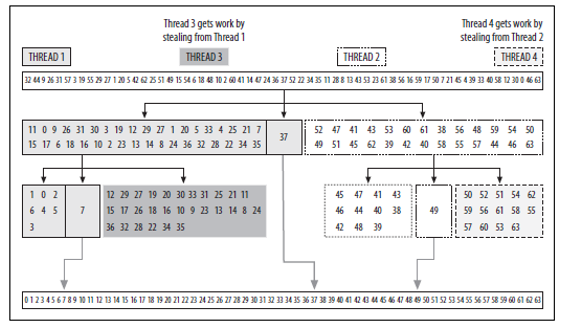
\includegraphics[width=\linewidth]{../../../../modules/reports/parshina_s_quick_sort/picture8.png}
			\captionof{figure}{Третий и четвертый потоки «украли» для себя работу} \\[0.5pt]
		\end{center}    
		
		\begin{center}
			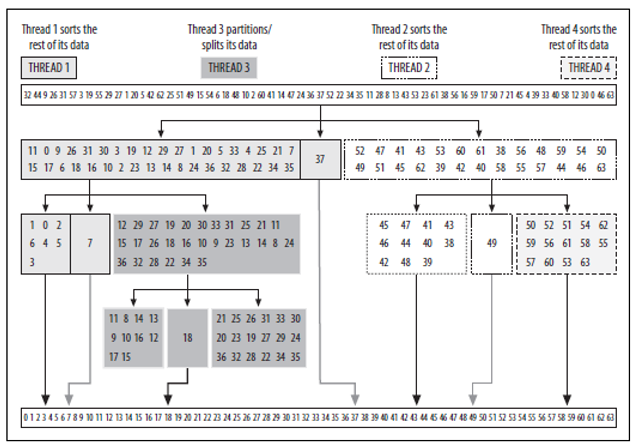
\includegraphics[width=\linewidth]{../../../../modules/reports/parshina_s_quick_sort/picture9.png}
			\captionof{figure}{Некоторые нагрузки разделяются, пока другие потоки заканчивают работу} \\[0.5pt]
		\end{center}
		
		\begin{center}
			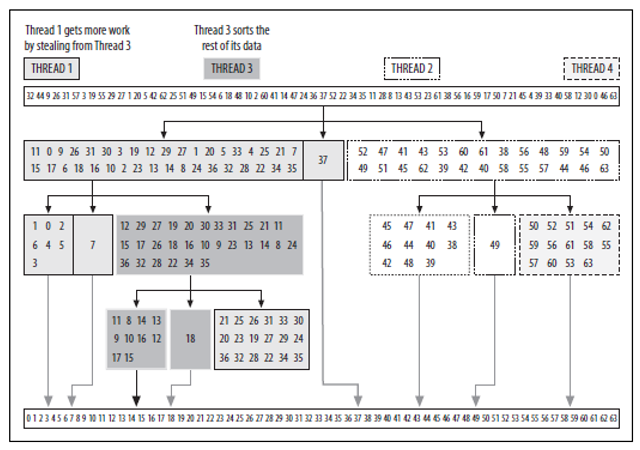
\includegraphics[width=\linewidth]{../../../../modules/reports/parshina_s_quick_sort/picture10.png}
			\captionof{figure}{Первый поток <<украл>> данные для себя, третий поток закончил} \\[0.5pt]
		\end{center}    
		
		\begin{center}
			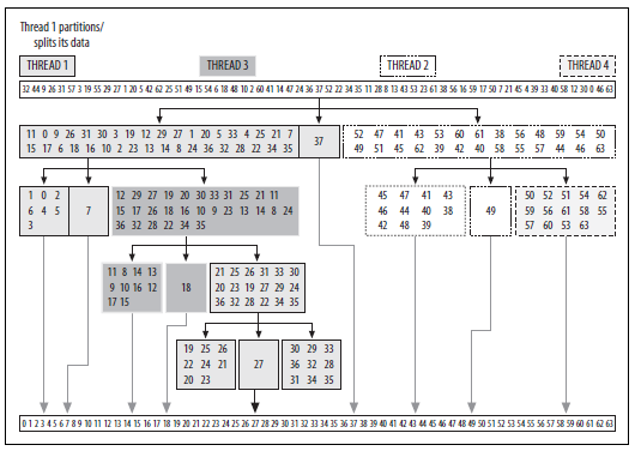
\includegraphics[width=\linewidth]{../../../../modules/reports/parshina_s_quick_sort/picture11.png}
			\captionof{figure}{Первый поток еще разделяет работу} \\[0.5pt]
		\end{center}    
		
		\begin{center}
			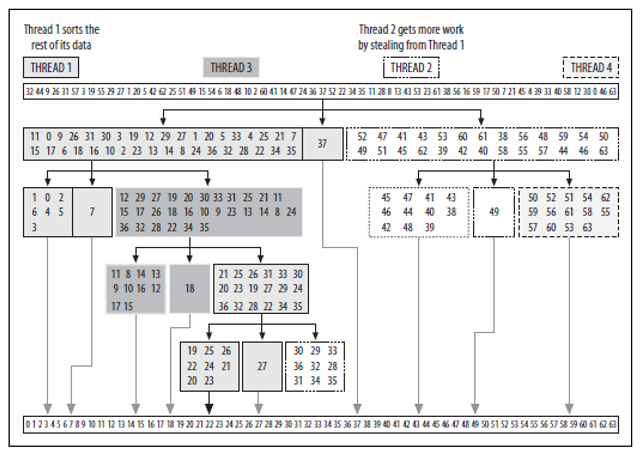
\includegraphics[width=\linewidth]{../../../../modules/reports/parshina_s_quick_sort/picture12.png}
			\captionof{figure}{Второй поток <<крадет>> работу, первый поток закончил} \\[0.5pt]
		\end{center}    
		
		\begin{center}
			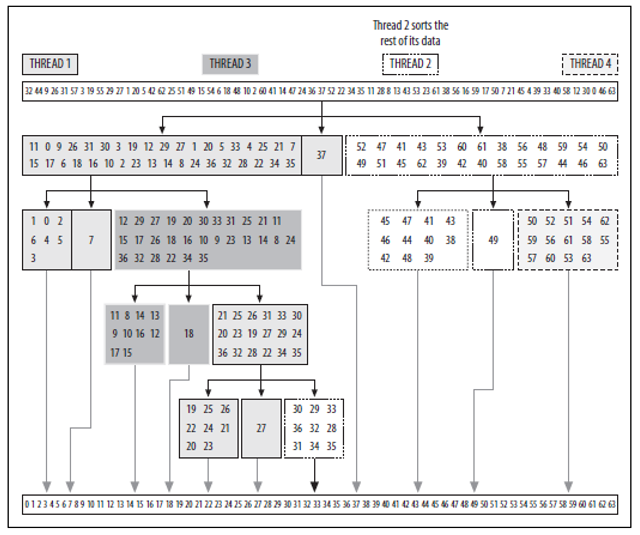
\includegraphics[width=\linewidth]{../../../../modules/reports/parshina_s_quick_sort/picture13.png}
			\captionof{figure}{Когда закончит второй поток, все закончат свою работу} \\[0.5pt]
		\end{center}    
		
		\par Рассмотрим подробнее программные возможности и реализацию быстрой сортировки. Полный код программы представлен в приложении А. Для начала работы с библиотекой необходимо подключить заголовочный файл \#include <tbb%/%tbb.h>.
		\par Библиотека Intel TBB имеет следующие классы для распараллеливания циклов с известным числом повторений, аналогичных циклов с редукцией, циклов с условием, рекурсии. Также библиотека содержит потокобезопасные контейнеры (очередь, хеш-таблица, вектор), операторы выделения динамической памяти и примитивы синхронизации. Для использования вышеперечисленных объектов должен быть инициализирован хотя бы один экземпляр класса tbb::task\_scheduler\_init. Он позволяет создавать потоки и структуры, необходимых планировщику потоков для работы. Прототип конструктора класса task\_scheduler\_init(int number\_of\_threads = automatic). Это непосредственная активация экземпляра класса с автоматическим (рекомендуемым) числом потоков. 
		\par По умолчанию лучше оставлять параметр количества потоков как automatic, так как планировщик потоков библиотеки TBB сам выделяет оптимальное число потоков. В некоторых источниках указано, что даже сам планировщик до некоторых пор не располагает информацией о числе потоков, на компьютере могут выполняться другие процессы и эта процедура может быть вложена в другие параллельные процедуры.
		\par Известно, что библиотека Intel TBB позволяет писать параллельные программы на уровне логических задач, а не на уровне работы напрямую с потоками. Для этого введено понятие логической задачи tbb::task. Это базовый класс, который наследуется всеми пользовательскими задачами. 
		\par Каждый поток имеет свой пул готовых к выполнению задач. Пул является динамическим массивом списков, которые обрабатываются в виде стека («last in first out»). Задачи на i-том уровне порождаются задачами уровня i-1. Поток выполняет задачи из самого нижнего непустого списка из массива списков. Если все списки пусты, то поток случайным образом «забирает» задачи, расположенные в наиболее низком списке у других потоков – «крадет» работу у других потоков.
		\par Каждая задача имеет owner – поток, который будет ее выполнять, parent – родитель задачи, у которого показатель refcount уменьшится на 1, когда эта задача завершит свое выполнение, depth – глубина задачи в пуле и refcount – число детей задачи. Три главных атрибута задачи (parent, depth, refcount).
		\par Задача task содержит главный метод task execute, в котором и приведены вычисления, после чего возвращается указатель на следующую к выполнению задачу. В данной задаче метод возвращает return NULL, это значит, что из пула готовых к выполнению задач выбирается новая.
		\par Таким образом, последовательность действий после назначения планировщиком потоку задачу на выполнение:
		
		\begin{enumerate} 
			\item запуск task::execute и ожидание его завершения;
			
			\item если не был вызван один из методов вида task::recycle\_*, то если parent не NULL, то parent->refcount уменьшается на единицу, а если parent->refcount становится равным 0, то задача parent помещается в пул готовых к выполнению;
			
			\item вызов деструктора задачи;
			
			\item освобождение памяти под задачей;
			
			\item если был вызван один из методов task::recycle\_*, то задача повторно добавляется в пул готовых к выполнению.
		\end{enumerate}
		
		\par В программном коде быстрой сортировки Хоара с простым слиянием реализован главный метод void qHoareSortTbb(double* arr, int n), в котором создается корневая или главная задача методом tbb::task::allocate\_root() типа qHoareSortTask с атрибутами (NULL, depth,0). Для запуска главной задачи необходимо использовать метод task::spawn\_root\_and\_wait.
		\par Класс qHoareSortTask – публичный класс типа tbb::task, который содержит приватные, доступные только внутри класса, переменные указателя на начало массива double* arr и его левый и правый конец int left\_index, right\_index. Конструктор класса реализован уже в публичной «секции класса» qHoareSortTask(double* arr1, int left\_index1, int right\_index1) : arr(arr1), left\_index(left\_index1), right\_index(right\_index1) {}. 
		\par Проанализируем основной метод task* execute(). Для начала введен минимальный порог, ниже которого параллельный алгоритм превращается в последовательную сортировку, то есть нет смысла распараллеливать быструю сортировку Хоара с количеством элементов меньше, чем 12 и, соответственно, применяем метод, написанный в первой лабораторной работе qHoareSort(arr, left\_index, right\_index). В случае большего количества элементов для удобства вставляем программный код разбиения Хоара непосредственно в метод execute. 
		\par Для удобства работы с набором задач Intel TBB поддерживает класс tbb::task\_list, который является  контейнером задач. Класс task\_list содержит два основных метода: push\_back – положить задачу в конец списка и pop\_front – достать задачу с удалением из начала списка. Как говорилось ранее, после разбиения Хоара необходимо рекурсивно доупорядочить 2 подмассива: от начала массива до крайнего правого индекса, на котором остановилось разбиение и от крайнего левого индекса, на котором завершилось разбиение Хоара до конца массива с проверкой соответствующих условий if (left\_index < right && right\_index > left).  В соответствии с этим в лист задач нужно положить 2 задачи методом push\_back: tasks\_list.push\_back(*new(tbb::task::allocate\_child()) qHoareSortTask(arr, left, right\_index)); tasks\_list.push\_back(*new(tbb::task::allocate\_child()) qHoareSortTask(arr, left\_index, right)).
		\par При выполнении обоих условий, необходимо назначить атрибут главной задачи set\_ref\_count(3), то есть 2 задачи, приведенные выше и находящиеся в листе +1: task::spawn\_and\_wait\_for\_all(tasks\_list) – добавить список задач tasks\_list в очередь готовых к выполнению и дождаться завершения всех подчиненных задач.
		\par В случае выполнения одного из условий if (left\_index < right) или if (left\_index >= right), то у корневой задачи атрибут set\_ref\_count(2) становится равным 2: соответствующая задача task::spawn\_and\_wait\_for\_all(*new(tbb::task::allocate\_child()) qHoareSortTask(arr, left\_index, right)) или task::spawn\_and\_wait\_for\_all
		(*new(tbb::task::allocate\_child()) qHoareSortTask(arr, left, right\_index)) + 1.
		\par При этом метод tbb::task::allocate\_child() позволяет создать подчиненную для корневой задачу типа qHoareSortTask с атрибутами (HoareSort, depth+1,0). При этом у корневой задачи HoareSort атрибуты меняются на (NULL,depth,refcount+1). Метод task::spawn\_and\_wait\_for\_all(tbb\& child) – добавить задачу в очередь готовых к выполнению задач и дождаться завершение всех подчиненных задач. 
		
		\newpage
		%--------------------------------------------------------------------------------
		%	РЕЗУЛЬТАТЫ ЭКСПЕРИМЕНТОВ, ОПИСАНИЕ ПОДТВЕРЖДЕНИЯ КОРРЕКТНОСТИ
		%--------------------------------------------------------------------------------
		\section{Результаты экспериментов}
		
		\par Все эксперименты проводятся на компьютере со следующими физическими характеристиками: процессор	Intel(R) Core(TM) i5-7200U CPU $@$ 2.50GHz, 2701 МГц, ядер: 2, логических процессоров: 4, установленная оперативная память (RAM) - 8,00 ГБ, кэш L1 - 128 КБ, кэш L2 - 512 КБ, кэш L3 - 3,0 МБ. 
		\par Эксперименты проводятся с количеством элементов n = 10, 1000, 10000, 100000, 1000000, 10000000, 100000000. Время в таблице представлено в секундах с различным числом элементов массива, количеством потоков и с использованием рассмотренных библиотек и рассчитано как среднее значение в результате проведения нескольких (5-20) тестов подряд.
		
		\begin{table}[h!]
			\caption{Результаты проведения экспериментов}
			\centering
			\begin{tabular}{|p{2.6cm}|p{2.8cm}|p{2.6cm}|p{2.6cm}|p{2.8cm}|}
				\hline
				
				Количество элементов n & Serial version, s & OpenMP version 2 threads, s & OpenMP version 4 threads, s & TBB version automatic number of threads, s \\ \hline
				
				100 & 3,11499E-06 & 0,000279235 & 0,000510855 & 0,0001337 \\ \hline
				
				1000 & 0,000039525 & 0,000180415 & 0,00068165 & 0,0003092 \\ \hline
				
				10000 & 0,00068513 & 0,00069723 & 0,000962585 & 0,0014534 \\ \hline
				
				100000 & 0,00839589 & 0,00534672 & 0,00463208 & 0,0048614 \\ \hline
				
				1000000 & 0,0921553 & 0,0586189 & 0,0486147 & 0,0454365 \\ \hline
				
				10000000 & 0,910147 & 0,607848 & 0,463434 & 0,464021 \\ \hline
				
				100000000 & 9,00256 & 5,97773 & 4,72149 & 4,57685 \\ \hline
				
			\end{tabular}
		\end{table}
		
		\begin{center}
			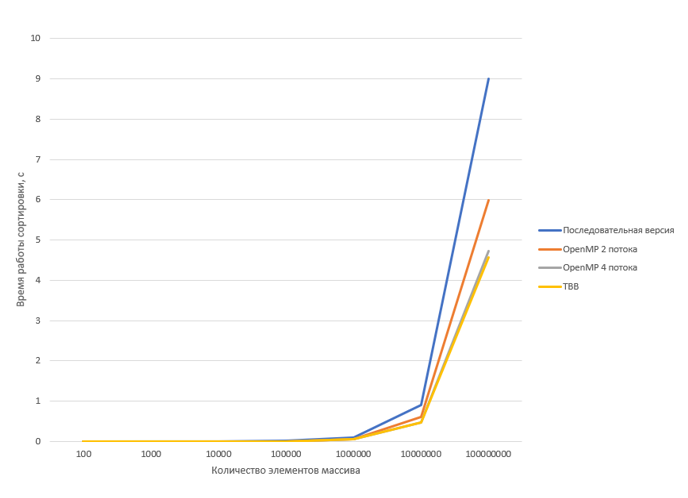
\includegraphics[width=\linewidth]{../../../../modules/reports/parshina_s_quick_sort/picture14.png}
			\captionof{figure}{Сравнительный график времен работы быстрой сортировки всех версий программы} \\[0.5pt]
		\end{center}    
		
		\begin{table}[h!]
			\caption{Ускорения OpenMP и TBB версий}
			\centering
			\begin{tabular}{|p{3.5cm}|p{4cm}|p{4cm}|p{3.8cm}|}
				\hline
				
				Количество элементов n & Serial/OpenMP 2 потока & Serial/OpenMP 4 потока & Serial/TBB  \\ \hline
				
				100 & 0,011155 & 0,006098 & 0,023298 \\ \hline
				
				1000 & 0,219078 & 0,057984 & 0,12783 \\ \hline
				
				10000 & 0,982646 & 0,711761 & 0,471398 \\ \hline
				
				100000 & 1,570288 & 1,812553 & 1,727051878 \\ \hline
				
				1000000 & 1,572109 & 1,895626 & 2,028222 \\ \hline
				
				10000000 & 1,497327 & 1,963919 & 1,961435 \\ \hline
				
				100000000 & 1,506016 & 1,90672 & 1,966977 \\ \hline
				
			\end{tabular}
		\end{table}
		
		\begin{center}
			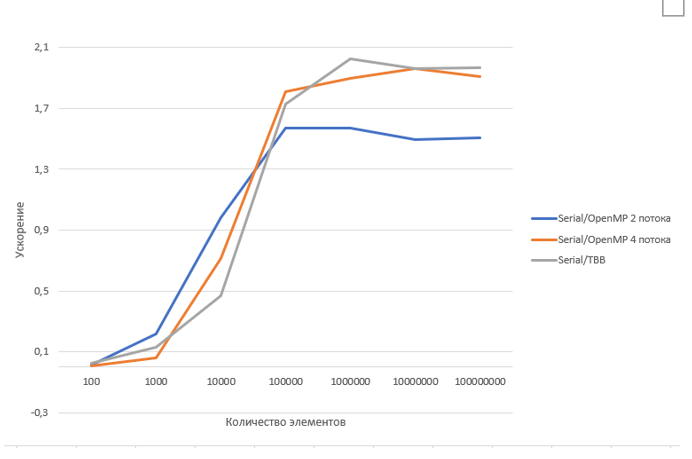
\includegraphics[width=\linewidth]{../../../../modules/reports/parshina_s_quick_sort/picture15.png}
			\captionof{figure}{График ускорений всех версий быстрой сортировки относительно последовательной} \\[0.5pt]
		\end{center} 
		
		\newpage
		%--------------------------------------------------------------------------------
		%	ВЫВОДЫ ИЗ РЕЗУЛЬТАТОВ ЭКСПЕРИМЕНТОВ
		%--------------------------------------------------------------------------------
		\section{Выводы из результатов экспериментов}
		
		\par В ходе экспериментов было проведено вычисление и сравнение времени работы последовательной версии, параллельных OpenMP с 2 и 4 потоками и Intel TBB с автоматически назначенным числом потоков версий. Была проведена проверка на корректность и выявлен тот факт, что все версии быстрой сортировки Хоара с простым слиянием с определенного количества (100000) элементов массива дают как минимум полуторное ускорение.
		\par Введем некоторые показатели эффективности параллельного алгоритма. Пусть величина n будет использована для параметризации вычислительной задачи и может пониматься как характерная размерность или количество входных данных. 
		\par Ускорение (speedup), получаемое при использовании параллельного алгоритма для p процессоров, по сравнению с последовательным вариантом выполнения вычислений определяется как Sp(N) = T1(n)$/$ Tp(n), где T1(n) – время выполнения последовательной быстрой сортировки n элементов, Tp(n) – время выполнения параллельного алгоритма. 
		\par Эффективность пользования параллельным алгоритмом определяется как Ep(n) = Sp(n)$/$p = T1(n)$/$(p*Tp(n)). 
		Из рассмотренных выше соотношений следует, что в лучшем случае, при неограниченном числе ресурсов, теоретически Sp(n) = p, Ep(n) = 1. Повышение качества параллельных вычислений по одному из показателей может привести к ухудшению по другому, то есть они являются взаимно противоречивыми.
		\par Может возникнуть такая ситуация, когда ускорение превысит по величине числе процессоров, тогда говорят о сверхлинейном ускорении. Одной из причин такого явления является неравноправность выполнения последовательной и параллельной программ. Например, если на одном процессоре оказывается недостаточно оперативной памяти для хранения всех обрабатываемых данных и необходимо будет использовать более медленную внешнюю память.
		\par Еще одной характеристикой является оценка стоимости вычислений, которая вычисляется как произведение времени выполнения параллельного кода и числа процессоров Cp = p*Tp. Тогда стоимостно-оптимальный параллельный алгоритм определяется как алгоритм, стоимость которого пропорциональна времени T1 выполнения наилучшего последовательного алгоритма. 
		\par Если зафиксировать число p процессоров и установить T1 = n-1, Tp = (n-1)$/$p + p, тогда ускорение, эффективность и стоимость параллельного алгоритма:
		\begin{center}
			\par Sp(n) = T1(n)$/$Tp(n) = (n-1)$/$((n-1)/p+p) -> p при n->$\infty$
			\par Ep(n) = Sp(n)$/$p = (n-1)$/$(n-1+p2)->1 при n->$\infty$
			\par Cp(n) = p*Tp(n) = n-1+ $p^2$
		\end{center}
		
		\par При n->$\infty$ алгоритм является стоимостно-оптимальным, то есть с теоретической точки зрения, с ростом характерной размерности n решаемые задачи распараллеливаются более эффективно. 
		\par С точки зрения задачи быстрой сортировки Хоара с простым слиянием по таблицам 1 и 2 можно отследить, что с увеличением n увеличивается ускорение относительно последовательной версии, а конкретнее параллелизм при n = 100-1000 не имеет смысла и параллельные алгоритмы для быстрой сортировки неэффективно использовать для маленького числа элементов относительно «масштабов» быстрой сортировки. С числа элементов n = 100.000 и вплоть до 100.000.000 достигается ускорение от 1,5 до 2,3 относительно последовательного времени. 
		
		\begin{spacing}{0.5}
			\par Максимальное ускорение достигается в TBB версии с автоматическим числом потоков, определяемым планировщиком потоков, при увеличении до 50 элементов минимального порога, до которого массив будет сортироваться последовательной быстрой сортировкой Хоара:
		\end{spacing}
		
		\begin{lstlisting}[language=C++]
		task* execute() {
		int min_parallel_length = 50;
		if (right_index - left_index <= min_parallel_length) {
		qHoareSort(arr, left_index, right_index);
		} else { 
		// Parallel TBB Quick Hoare sort }
		\end{lstlisting}
		
		\par OpenMP версия на 4 потоках работает быстрее, чем на 2 потоках, даже с учетом того, что физических ядер на компьютере 2. Но при этом логических ядер 4 и нужно учитывать тот факт, на симметричных мультипроцессорных системах параллельный алгоритм для некоторых значений характерной размерности n задачи может лучше использовать ресурсы кэш-памяти имеющихся процессоров. Как уточнялось ранее, если размер сортируемого массива велик настолько, что массив не может быть полностью помещен в кэш, то по мере выполнения последовательного алгоритма быстрой сортировки будет происходить чтение данных из оперативной памяти в кэш. Количество чтений определяется порядком выполнения итераций алгоритма и разницей в объеме данных для сортировки и объеме кэш. Таким образом, за счет обращения к кэшу параллельный алгоритм на 4 потоках и 4 логических ядрах работает в 1,3-1,5 раза быстрее, чем на 2 потоках.
		\par В описании TBB версии (пункт 4.2) уже приведено объяснение момента с автоматическим назначением числа потоков. Добавляя к той информации, в некоторых статьях планировщик потоков назначает столько потоков, сколько ядер в системе.
		\par Судя по таблице 2, параллельный алгоритм с использованием библиотеки Intel TBB на большом количестве элементов работает эффективнее, чем OpenMP версия на 2 потоках и в некоторых случаях быстрее, чем OpenMP на 4 потоках, однако в пределах 100.000-1.000.000 и OpenMP, и TBB дают примерно одинаковые результаты, а до 1000 элементов TBB работает примерно в 2 медленнее, чем OpenMP на 2 потоках. 
		\par Также эмпирически выяснено, что метод простого слияния void Simple\_Fusion(double * arr, int n, int m) – метод, в котором осуществляется слияние двух уже отсортированных частей массив в один упорядоченный массив в OpenMP версии при двукратном увеличении потоков замедляется в полтора раза, а сама быстрая сортировка Хоара в этой версии выполняется 
		последовательно.
		\par Заканчивая рассуждения над результатами экспериментов, хочется отметить, что для того, чтобы хоть что-то запустить в параллельное вычисление, естесственно нужно создавать потоки. Процесс создания потоков требует времени. Синхронизация потоков аналогично требует времени, потому распараллеливание даёт прирост только в том случае, когда экономия времени за счёт параллельного исполнения превышает накладные расходы по обслуживанию потоков. Иначе говоря, прирост производительности будет только на большом объёме данных. Это правило относится ко всем рассмотренным методам распараллеливания.
		
		\newpage
		%--------------------------------------------------------------------------------
		%	ЗАКЛЮЧЕНИЕ
		%--------------------------------------------------------------------------------
		
		\centerline{\section*{Заключение}}
		\addcontentsline{toc}{section}{Заключение}
		
		\par В течение семестра было выполнено несколько лабораторных работ, направленных на теоретическое изучение одного из самых популярных и часто используемых для больших объемов данных вида сортировки: быстрой сортировки Хоара с простым слиянием, а также на программную реализацию последовательной и двух параллельных версий этой сортировки с помощью технологий OpenMP и Intel Threading Building Blocks. 
		\par В процессе тестирования и проведения экспериментов было проверена корректность результатов и правильность программного кода и, соответственно, успешное достижение всех целей лабораторных работ. Параллельные версии показывают ускорение в диапазоне от 1,5 от 2,3 по сравнению с последовательным временем выполнения быстрой сортировки. При сравнении параллельных алгоритмов друг с другом было выяснено, что самым эффективным способом распараллеливания быстрой сортировки Хоара с простым слиянием является использование библиотеки шаблонов Intel TBB с автоматическим назначением числа потоков. 
		\par Помимо кода программы были разработаны и успешно запущены google тесты с помощью библиотеки для модульного тестирования на языке С++ Google C++ Testing Framework, которые отражают корректную работу методов и классов, реализованных в рамках лабораторных работ. 
		
		\newpage
		%--------------------------------------------------------------------------------
		%	СПИСОК ЛИТЕРАТУРЫ
		%--------------------------------------------------------------------------------
		
		\centerline{\section*{Список литературы}}
		\addcontentsline{toc}{section}{Список литературы}
		
		\begin{enumerate} 
			\item Гергель В.П. Современные языки и технологии параллельного программирования / Гергель В.П. - Издательство Московского Университета, 2012. - 408 с.
			
			\item Лабутина А.А. Учебный курс «Введение в метод параллельного программирования» / А.А.Лабутина - Нижегородский государственный университет им. Н.И.Лобачевского, межфакультетская магистратура по системному и прикладному программированию для многоядерных компьютерных систем, 2007 г. – 43 с.
			
			\item Андрейченко Д.К. Теоретические основы параллельного программирования / Андрейченко Д.К., Велиев В.М., Ерофтиев А.А., Портенко М.С. – Саратов, 2015 г. – 282 с.
			
			\item Федотов А. Обзор библиотеки Intel TBB / Федотов А. - SSG/DPD/TCAR/Threading Runtimes, 2017 – 79 с.
			
			\item Мееров И.Б. Инструменты параллельного программирования для систем с общей памятью $/$ Мееров И.Б., Сысоев А.В., Сиднев А.А. – Нижегородский государственный университет им. Н.И.Лобачевского, Факультет Вычислительной математики и кибернетики 2009 – 172 с.
			
			\item Вирт Н. Алгоритмы и структуры данных $/$ Вирт Н. - Издательство Мир, 1989, 360 стр.
			
			\item Антонов А.С. Параллельное программирование с использованием технологии OpenMP: Учебное пособие $/$ Антонов А.С. – М.: Изд-во МГУ, 2009. – 77 с. 
			
			\item Параллельные задачи (tasks) OpenMP [электронный ресурс] – условия доступа:  https://pro-prof.com/archives/1220#page\_1
			
			\item Распараллеливание рекурсивных функций, используя OpenMP 3.0 task [электронный ресурс] – условия доступа: https://habr.com/en/company/intel/blog/99823/
			
			\item QuickSort [электронный ресурс] – условия доступа: https://www.geeksforgeeks.org/quick-sort/
			
			\item Reinders J. Intel Threading Building Blocks / Reinder J. – O’Reilly Media. Inc. 2007 – 319 с.
			
			\item Антонов А.С. Технологии параллельного программирования MPI и OpenMP / Антонов А.С. – Москва: Издательство МГУ, 2012- 344 с.
			
			\item Быстрая сортировка [электронный ресурс] – условия доступа: http://kvodo.ru/quicksort.html
			
			\item Быстрая сортировка. Материал из Википедии – свободной энциклопедии [электронный ресурс] – условия доступа: https://ru.wikipedia.org/wiki/Быстрая\_сортировка
			
			\item Parallel Quick Sort. Центр суперкомпьютерных технологий. Нижегородский государственный университет имени Н.И.Лобачевского – свободной энциклопедии [электронный ресурс] – условия доступа: http://www.hpcc.unn.ru/?dir=1030
			
		\end{enumerate}
		
		\newpage
		%--------------------------------------------------------------------------------
		%	ПРИЛОЖЕНИЕ А. КОД ПРОГРАММЫ
		%--------------------------------------------------------------------------------
		\begin{spacing}{0.5}
			\centerline{\section*{Приложение А}} 
			\addcontentsline{toc}{section}{Приложение А}
		\end{spacing}
		\centerline{(обязательное)}
		\centerline{\bfseriesКод программы} 
		
		\par Исходный код трех лабораторных работ.
		
		\par Первая лабораторная работа <<Последовательная версия быстрой сортировки Хоара с простым слиянием>>
		\lstinputlisting[language=C++, caption=Последовательная версия. Заголовочный файл]{../../../../modules/task_1/parshina_s_quick_sort/quick_sort.h}
		\lstinputlisting[language=C++, caption=Последовательная версия. Cpp файл]{../../../../modules/task_1/parshina_s_quick_sort/quick_sort.cpp}
		\lstinputlisting[language=C++, caption=Последовательная версия. Google Tests]{../../../../modules/task_1/parshina_s_quick_sort/main.cpp}
		
		
		\par Вторая лабораторная работа <<OpenMP версия быстрой сортировки Хоара с простым слиянием>>
		\lstinputlisting[language=C++, caption=OpenMP версия. Заголовочный файл]{../../../../modules/task_2/parshina_s_quick_sort/quick_sort.h}
		\lstinputlisting[language=C++, caption=OpenMP версия. Cpp файл]{../../../../modules/task_2/parshina_s_quick_sort/quick_sort.cpp}
		\lstinputlisting[language=C++, caption=OpenMP версия. Google Tests]{../../../../modules/task_2/parshina_s_quick_sort/main.cpp}
		
		
		\par Третья лабораторная работа <<TBB версия быстрой сортировки Хоара с простым слиянием>>
		\lstinputlisting[language=C++, caption=TBB версия. Заголовочный файл]{../../../../modules/task_3/parshina_s_quick_sort/quick_sort.h}
		\lstinputlisting[language=C++, caption=TBB версия. Cpp файл]{../../../../modules/task_3/parshina_s_quick_sort/quick_sort.cpp}
		\lstinputlisting[language=C++, caption=TBB версия. Google Tests]{../../../../modules/task_3/parshina_s_quick_sort/main.cpp}
		
	\end{spacing}
	
\end{document}